\chapter{Das Kampfsystem}
Ein zentrales Element des Spiels bildet das Kampfsystem. Karten können während des Kampfes ausgespielt und so für unterschiedlichste Aktionen eingesetzt werden. Als Faustregel gilt: Desto höher der Kartenwert, desto besser ist sie.

\section{Die Darstellung}
Um den Kampf dynamisch darzustellen und die verschiedenen Distanzregeln flüssig anwenden zu können, sollten die Kreaturen durch Marker oder Miniaturen dargestellt werden. Von oben betrachtet sollten ihre Bases in etwa kreisförmig und nicht größer als eine Kartenbreite sein. Um die Situation eindrucksvoll darzustellen, könnt ihr versuchen Minitauren in passenden Größenverhältnissen, gebasteltes Gelände und vielleicht sogar eine Spielmatte zu nutzen. In \textit{Ludus Mortis} wird ein freies Bewegungssystem genutzt, womit Schachbrettmuster und Hexerfeldmatten überflüssig werden und den Spielern eine größere Auswahl an Möglichkeiten offensteht um ihre Vorstellungen von einem spannenden Kampf auszuleben. Abhängig von den Größen der Marker einigen sich die Spieler mit dem Spielleiter auf ein Einheiten zur Bestimmung von Distanzen. Auch wenn es verlockend sein mag Distanzen in Kartenbreiten zu messen, hat sich wärend einigen Probespielen die Schwirigkeit mit großen Distanzen herausgestellt und wir empfehlen dem Spieler auf ein Herkömmliches System, wie 1 Zoll oder 2 cm pro Meter, umzusteigen.


\section{Der Kampfablauf}
Der Ablauf eines Kampfes vollzieht sich immer in Kampfrunden. Wenn kein Gegner oder keine befreundete Kreatur mehr kampffähig ist, wird der Kampf abgeschlossen und gilt entweder als gewonnen oder verloren. Jede Kampfrunde setzt sich aus 4 aufeinanderfolgenden Phasen zusammensetzt:

\begin{enumerate}
    \item Der Initiativzug
    \item Das Kartenziehen 
    \item Aktionsrunden 
    \item Ende der Kampfrunde
\end{enumerate}

\subsection*{1. Der Initiavivzug}
Jeder am Kampf beteiligter Charakter zieht die oberste Karte seines Kartenstappels. Die Addition aus dem Kartenwert und dem Grundwert der Initiative eines Charakters, bildet den Initiativwert für die Kampfrunde.

\subsection*{2. Das Kartenziehen}
Jeder Spielercharakter zieht bei diesem Schritt verdeckt 5 Handkarten. Diese Karten bilden für die restliche Kampfrunde die Hand eines Spielers. Es ist nicht erlaubt anderen Spielern Auskunft über seine Hand zu geben. Der Spielleiter darf Spieler welche sich nicht an diese Regel halten mit ablegen von Karten o.Ä. abstrafen. Nicht Spielercharaktere ziehen keine Karten sondern haben Aktionspunkte.

\subsection*{3. Aktionsrunden}
In einer Aktionsrunde kann jeder Charakter eine Aktionsphase durchführen. Der Spieler darf eine freie Aktion und danach eine Aktion (Hauptaktion) ausführen. Die Reihenfolge, in welcher die Charaktere ihre Aktionsphase ausführen können, wird anhand der Initiative festgelegt. Es fängt die Kreatur an, welches den höchsten Initiativwert der Kampfrunde aufzuweisen hat. Anschließend geht es den Initativwerten folgend absteigend weiter. Ein Spielercharakter kann eine Aktionsphase nur dann durchführen, wenn der Spieler noch Handkarten hat. Andernfalls wird der Spieler übersprungen. Nicht Spielercharaktere benutzen anstelle von Handkarten, die oberste Karte des Gegnerdecks (besonders mächtige Kreaturen können ein eigenes Deck haben). Um ihre Aktionsanzahl zu regeln, besitzt jede Kreatur Aktionspunkte (AP), welche am Ende einer Kampfrunde wieder vollständig aufgefüllt werden. Die Anzahl der notwendigen Aktionspunkte ist aktionsabhängig. In der Regel entspricht jedoch ein AP einer Aktion.

\subsection*{4. Ende der Kampfrunde}
Sobald keine Kreatur mehr eine Aktionsphase durchführen kann oder will, wird die Kampfrunde beendet. Jetzt darf jede Kreatur eine Vergiftung und eine geistige Umnachtung ablegen, wie auch eine mögliche Blutung oder Besserung um 1 reduzieren. Sollte  mindestens ein gegnerischer Charakter noch kampffähig sein, beginnt nun eine neue Kampfrunde. Der Kampf endet somit sobald alle Gegner oder die ganze Spielergruppe kampfunfähig ist.


\section{Nah- \& Fernkampf}
Im Kampf wird zwischen Nahkampf und Fernkampf unterschieden.
Nahkampf Aktionen sind alle Waffen Angriffe die auf die Schlagen Aktion gehen, sowie Aktionen mit einer Reichweite von maximal 1 m oder die als Nahkampf gekennzeichnet sind. Fernkampf Aktionen sind die Waffen Angriffe die auf Werfen oder Schießen gehen und alle anderen Aktionen, die Angriffe mit einer Reichweite von über 1 m sind. Fernkampfaktionen können falls keine Mindestreichweite angegeben ist auch  im Nahkampf ausgeführt werden.
Sollte man sich in maximal 1 m Entfernung zu einer gegnerischen Kreatur befindet, gilt man zu ihr als “Im Nahkampf”. Eine Kreatur kann mit einer unbegrenzten Anzahl an Gegnern gleichzeitig im Nahkampf sein. Der Nahkampf löst sich auf, wenn sich keine feindliche Kreatur mehr innerhalb von einem Meter befindet. Dies ist in der Regel der Fall, wenn jene Kreatur entweder besiegt wurde oder eine der Parteien sich aus dem Nahkampf bewegt hat. Sollte sich die Kreatur eigenständig aus der Nahkampfreichweite zu einer andere Kreatur bewegen, so darf diese sofort einen Nahkampfangriff gegen die fliehende Kreatur ausüben. Dies bedeutet für Spieler in der Regel den Verlust einer Handkarte und für Nichtspielercharaktere den Verlust eines Aktionpunkts. 

\section{Aktionen}
Aktionen sind besondere Proben welche nicht mit der obersten Karte des Decks sondern mit einer Handkarte getätigt. Dabei hat jede Aktion andere Anforderungen und Effekte.

\subsection*{Angriffe: Schlagen, Schießen und Werfen}
Egal ob es sich um ein mächtigen Wareguard, einen flinken Menschen oder den geschickten Skriva handelt, sie alle haben die Möglichkeit aggressiv gegen ihre  Feinde vorzugehen. Alle "Standart"-Nahkampfangriffe mit Fäusten, Krallen, Schwänzen oder Zähnen werden im allgemeinen unter den Angriff \textit{Schlagen} zusammengefasst und sind zusammen mit \textit{Schießen} und \textit{Werfen} Aktionen die jeder Kreatur zustehen. Diese und alle Artenspezifischen Angriffsaktionen funktionieren nach dem selben Schema: Der Angreifer führt eine Probe durch, modifiziert diese ggf., dann führt der Verteidiger eine vergleichende Probe durch und sieht nach ob er Wunden, entsprechend der negativen Differenz, erleidet.

\subsection*{Verteidigung: Block, Ausweichen u.a}
Wenn du durch Angegriffen wirst bist du dem Schaden nicht wehrlos ausgesetzt sondern kannst dich auch Verteidigen.\\
Physischen Schaden wie auch Spiritschaden kannst du entweder Blocken oder Ausweichen. Dazu wendest du die dementsprechende Aktion an und reduzierst den Schaden um den Wert der Aktion. Den über geblieben Schaden erleidest du als Wunden, wenn kein Schaden übrig bleibt ist der Angriff erfolgreich Verteidigt. Für Giftschaden wird die Aktion Giftresistenz genutzt und der übrige Schaden äußert sich in Giftverletzungen. Ahnlich wird Psycheschaden durch die Aktion Mentaler Widerstand Verteidigt und äußert sich in Psycheverletzungen


\subsubsection*{Waffenboni}
Wenn eine Kreatur Waffen führt, so erhält sie in der Regelboni auf ihre Angriffe und kann häufig von größeren Reichweiten profitieren. Diese Werten sind im weiter hinten unter \textit{\nameref{waffen}} zu finden. Es ist Kreaturen gestattet zwei Einhandwaffen gleichzeitig zu führen und so mit ihren Gegner zu überraschen. Bei Angriffen mit zwei Waffen deckt der Angreifer nach seiner ersten Karte ein Karte von seinem Deck auf und darf sich dann entscheiden welche der beiden Karten und somit Waffen er nutzen möchte. Er muss jedoch bevor er die zweite Karte aufdeckt den Karten bereits jeweils eine der aktiven Waffen zuweisen.

\subsection*{Aktionen Verketten}
Eine weitere besondere Eigenschaft von Aktionen ist das Verketten, es ermöglicht starke Aktionskombination auf kosten von "Erschöpfung". Während eines Kampfes kann ein Spieler sich nach seiner Aktion entscheiden eine weitere Aktion auszuführen. Hierzu legt er, bevor er die zweite Aktion ausführt, eine Karte ab. Diese Vorgang nennt sich Verketten und kann nur einmal pro Aktionsrunde (pro Kreatur) genutzt werden.


\section{Schadensarten}
Ein 100 kg schwerer Hammer der deine Hand zertrümmert ist definitiv etwas anders, als ein Gift, dass nach und nach deine Glieder verschmilzt. Um verschiedene Schadenstypen behandeln zu können gibt es drei unterschiedliche Kategorien wie sich Schaden auswirken kann: Wunden, Gift oder Psyche. Im offenen Kampf werden euch zumeist Wunden zugefügt, wohingegen hinterhältige Wesen und Fallen gerne mal eure Giftresistenz und Psyche auf die Probe stellen. Außerdem kann deine Kreatur schwere Verletzungen erleiden, die dich permanent schwächen.

\subsection*{Wunden}
Das Wundenlimit gibt Auskunft über die generelle physische Verfassung deiner Kreatur und bildet den Kern der Gesundheit. Das Wundenlimit gibt an wie viele Wunden deine Kreatur erleiden kann bevor sie Kampfunfähig wird.
Eine Kreatur ist Kampfunfähig sobald die Wunden größer als das Wundenlimit sind. Gegnerische Kreaturen sind solange der Spielleiter keine anderen Pläne hat in dem Fall der Kampfunfähigkeit tot. Falls eine Kreatur Kampfunfähig wird erleidet sie sofort eine schwere Verletzung und kann keiene Aktionen wirken solange sie Kampfunfähig ist. Eine Kreatur ist dann nicht mehr Kampfunfähig, wenn die Wunden unter das Wundenlimit fallen.\\
Falls deine Kreatur die Hälfte des Wundenlimits oder mehr auf einmal an Wunden erleidet (über eine Aktion/Angriff) erhält sie auch eine schwere Verletzung.

\subsection*{Vergiftungen}
Sobald der maximum Giftwert einer Kreatur überschritten wird erleidet die Kreatur eine Vergiftung. Die Vergiftung ist eine Art Leiden das sich durch eine der Giftkarte ausdrückt. Somit gibt es viele verschiedene Vergiftungen. Eine (Gift-) Aktion kann eine spezielle Vergiftung vorgeben, falls dies der Fall ist kann nur die genannte Vergiftung über die Aktion verteilt werden, es sei den eine Auswahl liegt vor dann kann der Spieler bevor er Aktion durchführt das Gift ansagen. In allen anderen Fällen wird eine Giftkarte aus dem Gift Stapel gezogen oder vom Spielmeister ausgewählt.
Es kann (wenn die Aktion nichts anderes sagt) nur immer ein Gift pro Aktion verursacht werden. Giftschaden der den maximum Giftwert übersteigt wird für die nächste Vergiftung übertragen, nachdem der Giftwert nach einer Vergiftung zurückgesetzt wird.
Am Ende der Kampfrunde darf jede Kreatur eine Vergiftung von sich ablegen (egal welche).\\
Die Grundvergiftungen sind:

\begin{itemize}
    \item \textbf{Brennedes Gift:}\\
    Erleide Brennden in höhe des Toxinwertes der vergiftenden Kreatur.
    \item \textbf{Gefrierendes Gift:}\\
    Verdoppel die nächsten Wunden, die du erleidest, lege diese Karte ab. Dies lösst keine schweren Verletzungen aus.
    \item \textbf{Lähmendes Gift:}\\
    Dein Bewegungswert ist halbiert.
    \item \textbf{Reines Gift:}\\
    Erleide zu beginn deiner Aktionsphase 2 Wunden.
    \item \textbf{Schwächendes Gift:}\\
    Du hast -5 auf Kraft- und Blockenaktionen.
    \item \textbf{Verlangsamendes Gift:}\\
    Du hast -5 auf Geschick- und Ausweichaktionen.
\end{itemize}


\subsection*{Psyche}
Psyche wird analog wie Vergiftungen behandelt. Somit erleidet eine Kreatur eine geistige Umnachtung, sobald der maximale Psychewert überschritten wird.
Die geistige Umnachtung äußert sich ebenfalls als eine Art Leiden in der Form einer Karte. Solange keine spezifische Umnachtung vorgegeben ist wird eine der gleich genannten Umnachtungen durch den Spielmeister oder Zufall bestimmt.
Pro Aktion kann nur eine geistige Umnachtung pro Kreatur erzwungen werden, im falle des Auslösen einer Umnachtung wird der aktuelle Wert auf 0 gesetzt und alle überschüssigen Psychewunden neu drauf gerechnet.
Am Ende der Kampfrunde darf jede Kreatur eine geistige Umnachtung von sich ablegen (egal welche).\\
Die geistigen Umnachtungen sind:

\begin{itemize}
    \item \textbf{Innerer Konflikt:}\\
    Deine nächste Aktion musst du deinem inneren Konflikt widmen, wirf eine Karte ab und beende deine Aktionsphase.
    \item \textbf{Panische Flucht:}\\
    Bewege dich sofort Bewegung + 1 m von der Quelle der geistigen Umnachtung weg.  
    \item \textbf{Wie angewurzelt:}\\
    Du kannst dich nicht mehr Laufen. Nach deiner nächsten Aktionsphase endet der Effekt.
    \item \textbf{Lähmende Angst:}\\
    Für den Rest der Kampfrunde kannst du die Quelle deiner Angst nicht mehr als Ziel wählen.
    \item \textbf{Unter Schock:}\\
    Für den Rest der Kampfrunde agierst du immer als letzter in einer Aktionsrunde.
\end{itemize}

\subsection*{schwere Verletzungen}
Immer wenn eine Kreatur die Hälfte oder mehr ihrer maximalen Wunden auf einen Schlag verliert oder das Wundenlimit überschreitet erleidet sie eine schwere Verletzung. Jeder weitere Schaden der einer Kreatur zugefügt wird die bereits Wundernüber dem Wundenlimit hat, erleidet eine weiter schwere Verletzung.
Die ersten 3 schweren Verletzungen geben jeweils ein Malus von -1 auf alle Eigenschaften. Die vierte schwere Verletzung fügt einen weiteren diesmal spezifischen Malus hinzu, eine Auswahl ist in der folgenden Tabelle zu finden. Der Erzähler kann aus erzählerischen Gründen eine Auswählen die zur Situation passt, sonst kann auch zufällig ausgewählt werden.

Wenn eine spezifische schwere Verletzung gewählt wurde kann diese bis sie wieder geheilt wird in dem passenden Feld bei schweren Verletzungen festgehalten werden.
Die fünfte schwere Verletzung führt zum unmittelbaren Tod, der dann nicht noch verhindert werden kann.
Schwere Verletzungen heilen nicht über Nacht, eine Kreatur mit einer schweren Verletzung braucht viel Flege und vorallem Zeit um diese auszukurieren. 

\section{Der Tod}
Sobald eine Kreatur ihre 5te schwere Verletzung erleidet ist sie unverzüglich tot und kann nicht mehr von ihrem Tod bewahrt werden.
Manche taten von Kreaturen führen auch zu ihrem sofortigen Tod, wie z.B der Sprung eienes Menschen in ein Lavasee. Dies liegt im ermessen des Spielleiters, sollte jedoch nur die äußerste und letzte Massnahme sein.
Der Tod durch Krankheiten o.a kann auch ein gutes Storyelement bieten.

\section{Regeneration}
Mit der Zeit heilen die im Kampf erlittenen Wunden und auch schweren Verletzungen.
Um dies darzustellen hat jede Kreatur einen Regenerationswert. Der Regenerationswert entspricht der Zehnerstelle des Wundenmaximums oder Wundenmaximum durch 10. Bei einem Wundenmaximum unter 10 ist der Wert 1. Durch Fähigkeiten oder Ausrüstung kann sich dieser Wert noch erhöhen, aber nie größer als die Hälfte des Wundenmaximums sein.\\
Nach einem Kampf können alle überlebenden, damit auch alle Kampfunfähigen kurz durch schnaufen und Wunden in Höhe ihrer Regeneration heilen. Kampfunfähige brauchen dennoch etwas Zeit um wieder zu sich zu finden.
Ebenfalls trägt das Spiritfeld der heimlichen Lande zur einer schnellen Regeneration bei, für jede Stunde die man Rastet verringern sich die Wunden um den Regenerationswert.\\
Schwere Verletzungen brauchen dagegen mehr Fürsorge. Um eine schwere Verletzung auszukurieren brauch es Wochen oder einen Gelehrten der Medizin mit entsprechenden medizinischen Gütern und ein paar Tage. 

\clearpage
\section*{Liste der schweren Verletzungen}
\begin{table}[htpb]
    \centering
    \begin{tabular}{|c|c|c|}
        \hline
        \textbf{Bezeichnung} & \textbf{Effekt} & \textbf{Kartenwert}\\
        \hline
        \hline
         & &\\
        Beinbruch & Bewegungsreichweite halbiert & 2-5 \\
         & &\\
        \hline
         & &\\
        Denkfehler &  Ziehe eine Karte beim Kartenziehen weniger & 6-7 \\
         & &\\
        \hline
         & &\\
        Fähigkeitenschwund & Außsetzten einer passiven Fähigkeit & 8\\
         & &\\
        \hline
         & &\\
        Triefende Wunde & Wunden nehmen nicht mehr ab, können jedoch noch geheilt werden & 9-10\\
         & &\\
        \hline
         & &\\
        Krafteinbüßen & Halbiere deinen Karftwert & Bube \\
         & &\\
        \hline
         & &\\
        Geschwächt & Proben sind ein Schwierigkeitsgrad schwieriger & Dame\\ 
         & &\\
        \hline
         & &\\
        Spiritverlust & Du kannst keine Spiritaktionen nutzen & König-As\\
         & &\\
        \hline
    \end{tabular}
    \label{tab:schwere_Verletzungen}
\end{table}
\begin{figure}[b]
    \centering
    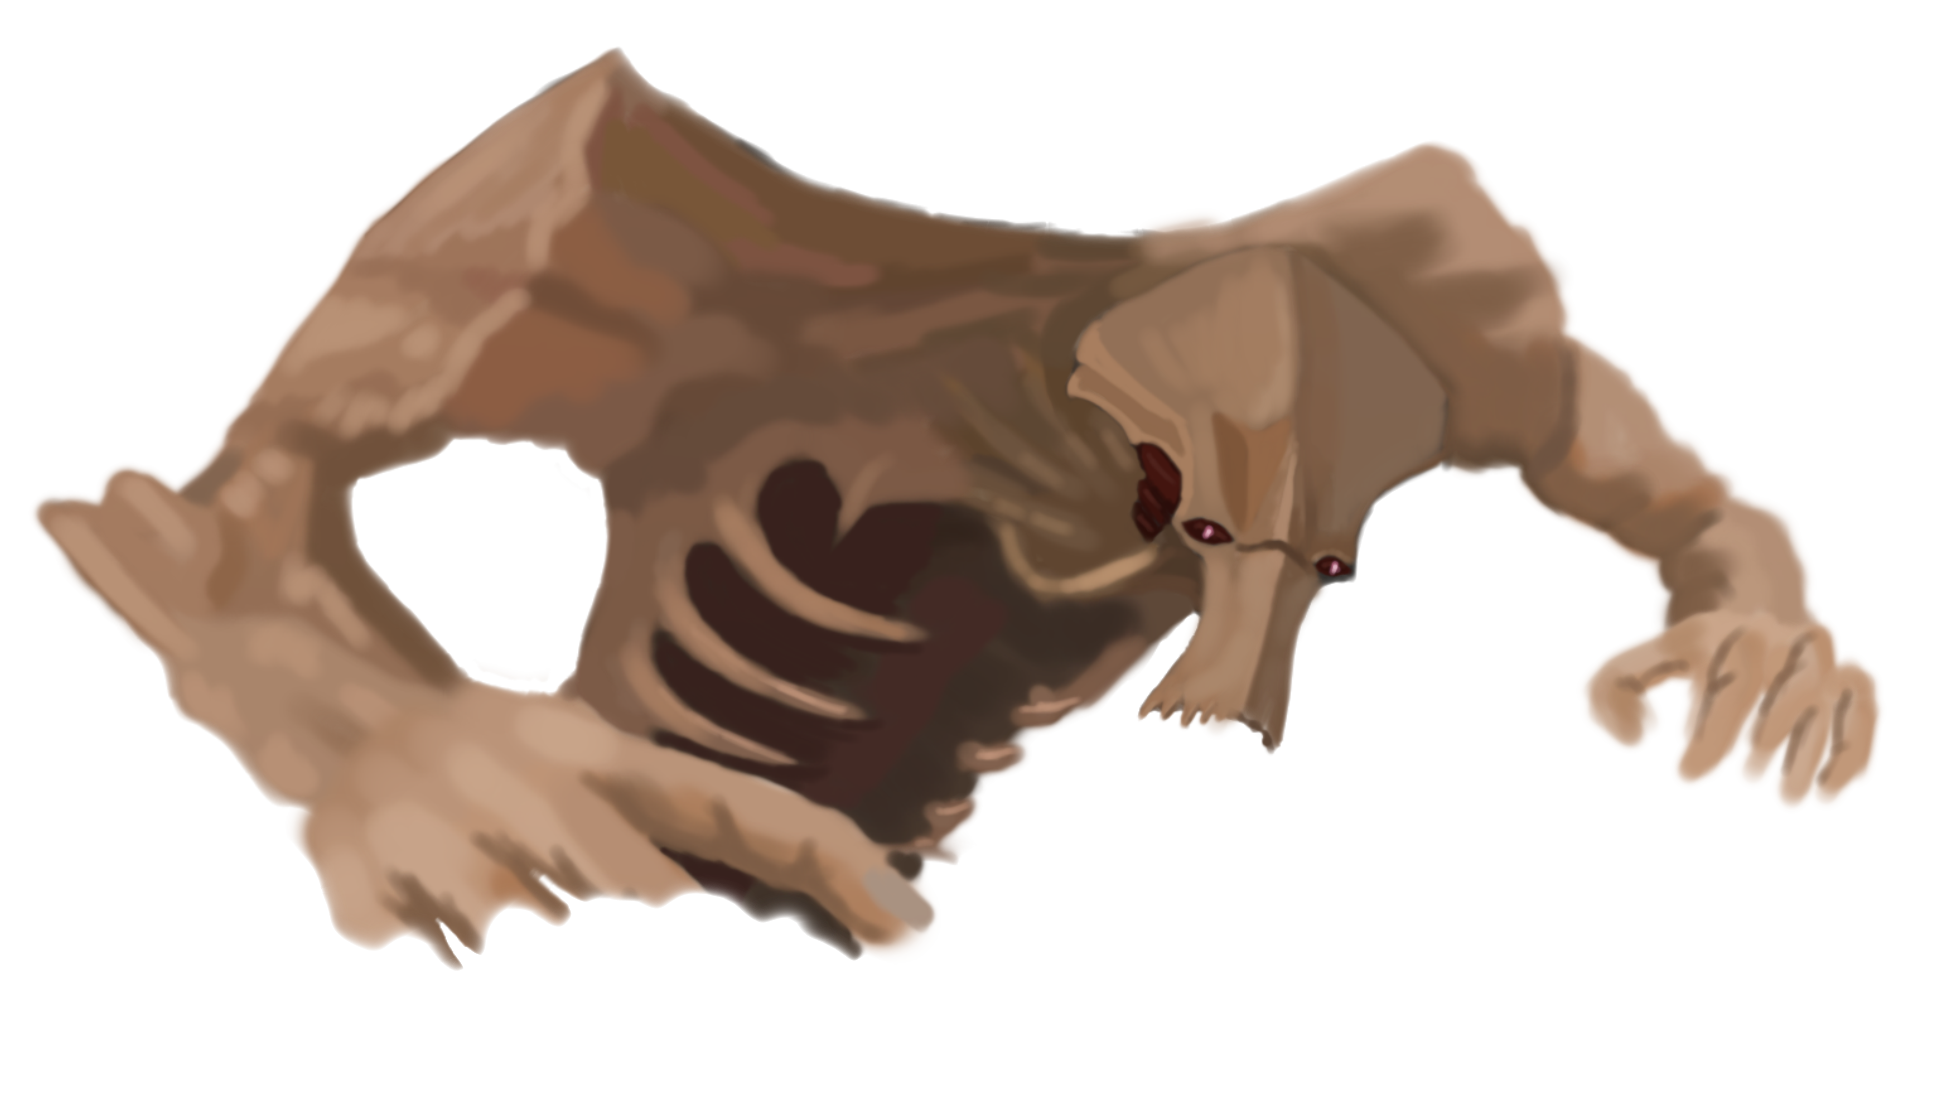
\includegraphics[width = 0.5\textwidth]{Pictures/Witchscreamer.png}
    \label{fig:Howler}
\end{figure}
